%
% The first command in your LaTeX source must be the \documentclass command.
\documentclass[sigchi]{acmart}
\usepackage{array}
\usepackage{graphicx}

%
% defining the \BibTeX command - from Oren Patashnik's original BibTeX documentation.
\def\BibTeX{{\rm B\kern-.05em{\sc i\kern-.025em b}\kern-.08emT\kern-.1667em\lower.7ex\hbox{E}\kern-.125emX}}
    
% Rights management information. 
% This information is sent to you when you complete the rights form.
% These commands have SAMPLE values in them; it is your responsibility as an author to replace
% the commands and values with those provided to you when you complete the rights form.
%
% These commands are for a PROCEEDINGS abstract or paper.
\copyrightyear{2025}
\acmYear{2025}
\setcopyright{acmlicensed}
\acmConference[SNA '25]{Social Network Analysis '24}{2024/25}{University of Pisa, Italy}
\acmBooktitle{Analisi dell'affinità musicale degli artisti di Last.fm}
\acmPrice{0.00}
%\acmDOI{10.1145/1122445.1122456}
%\acmISBN{978-1-4503-9999-9/18/06}

% end of the preamble, start of the body of the document source.
\begin{document}

%
% The "title" command has an optional parameter, allowing the author to define a "short title" to be used in page headers.
\title{Analisi dell'affinità musicale degli artisti di Last.fm}

%
% The "author" command and its associated commands are used to define the authors and their affiliations.
% Of note is the shared affiliation of the first two authors, and the "authornote" and "authornotemark" commands
% used to denote shared contribution to the research.
\author{Calogero Giudice}
\email{c.giudice@studenti.unipi.it}
\affiliation{%
  \institution{Student ID: 530155}
}

\renewcommand{\shortauthors}{Calogero Giudice}


% The abstract is a short summary of the work to be presented in the article.
\begin{abstract}
Questo progetto analizza una rete di artisti musicali del social network {\itshape \href{https://www.last.fm/home}{last.fm}} in base a dei coefficienti di similarità (Sample e Jaccard Ratios) che potrebbero rappresentare delle affinità a livello stilistico o di pubblico. Sono state esaminate sia le {\bfseries caratteristiche strutturali} della rete, procedendo a svolgere una previsione, in base ai Ratios menzionati in precedenza e al coefficiente di popolarità, su possibili aumenti o cali di popolarità futuri. \\ \\ Questi risultati possono rappresentare un {\bfseries modello} che potrebbe riflettersi nello scenario musicale odierno, fornendo nuovi studi e strumenti che possono essere utili a prevedere eventuali nuovi scenari. Infatti, possono esserci artisti emergenti che potrebbero godere di maggiore popolarità futura se ben collegati, con artisti di popolarità alta e collegati con ratio alti; allo stesso tempo, si potrebbero notare alcuni artisti ritenuti popolari che potrebbero avere un trend opposto e quindi in declino.\footnote{
{\bf Project Repositories}\\
\noindent Data Collection: \url{https://github.com/Kalo9603/2024_Giudice/tree/main/data_collection}\\
\noindent Network Analysis: \url{https://github.com/Kalo9603/2024_Giudice/tree/main/network_analysis}\\
\noindent Open Problem: \url{https://github.com/Kalo9603/2024_Giudice/tree/main/open_problem}\\
\noindent Report: \url{https://github.com/Kalo9603/2024_Giudice/tree/main/report}}
\end{abstract}


%
% Keywords. The author(s) should pick words that accurately describe the work being
% presented. Separate the keywords with commas.
\keywords{Social Network Analysis, musica, {\itshape Last.fm}, affinità, similarità, popolarità}


%
% This command processes the author and affiliation and title information and builds
% the first part of the formatted document.
\maketitle

\section{Introduzione}
Nell'epoca dell'affermazione dell'industria musicale digitale, piattaforme come {\itshape \href{https://www.last.fm/home}{last.fm}} offrono tanti dati sugli artisti musicali, sulle abitudini di ascolto degli utenti e sulle relazioni tra i singoli profili musicali (gli utenti, gli artisti, gli album, etc.). Gli artisti presenti nella piattaforma sono stati analizzati sotto una prospettiva di rete sociale: si possono ipotizzare così degli scenari, dei fenomeni interessanti: la similarità tra artisti, la popolarità degli stessi, l'affermazione di artisti emergenti o l'effetto contrario. \\ \\ L'analisi parte dalla costruzione di una rete basata su coefficienti di similarità; di questi ne sono stati individuati due:

\begin{itemize}
\item Il {\itshape Sample Ratio}, ovvero l’intensità del legame tra due artisti in base ai simili condivisi.
\item Lo {\itshape Jaccard Ratio}, ovvero l’affinità relativa all’insieme totale di simili.
\end{itemize}
Matematicamente, è molto più probabile che lo {\itshape Jaccard} sia inferiore del rispettivo {\itshape Sample}, poiché il denominatore del primo è sempre maggiore del secondo (a meno che tali denominatori non coincidono). \\ \\ In parallelo si è stimata la {\bfseries popolarità} degli artisti presenti nel dataset: per far ciò ci si è basati sullo {\bfseries Z-Index}, che mette in relazione il numero di ascoltatori e quello di ascolti. Ciò ha permesso di classificare gli artisti in tre classi: {\bfseries \itshape mainstream}, {\bfseries \itshape medio} ed {\bfseries \itshape emergente}; a questi ne sono stati affiancati altri tre: {\bfseries \itshape possibile mainstream}, {\bfseries \itshape possibile medio} e {\bfseries \itshape ritorno emergente} in base al trend di (de)crescita calcolato. \\ \\ L'obiettivo principale della seconda parte progetto è quello di identificare le caratteristiche strutturali degli artisti mainstream e di quelli emergenti ed, eventualmente, di prevedere un cambio di status in base a determinate metriche.


\section{Data Collection}

La raccolta dei dati da analizzare si è concentrata su tre fasi specifiche:
\begin{enumerate}
\item La generazione di un elenco di artisti in base agli artisti simili;
\item La creazione di una lista di archi che collegano due artisti se entrambi i coefficienti di similarità superano la soglia del $50\%$. Il {\itshape Sample Ratio} è calcolato rispetto al numero di simili condivisi, mentre lo {\itshape Jaccard Ratio} rispetto all'insieme totale dei simili;
\item Il successivo accostamento del numero di ascolti, di ascoltatori e il calcolo delle popolarità degli artisti.
\end{enumerate}
Gli elenchi degli artisti e degli artisti simili sono stati ottenuti per mezzo dell'API di {\itshape last.fm} e, tramite programmazione ad oggetti, sono state generate le altre liste. Nel complesso vi sono quattro file:

\begin{itemize}
\item {\itshape artists.csv}, una lista di 28\,870 artisti;
\item {\itshape links.csv}, un elenco di 98\,890 archi che collegano 11\,745 artisti (il 40.68\% del totale). A causa delle lunghe tempistiche è stato elaborato il dataset sul 64.26\% dei possibili archi totali (sono stati esaminati più di 267 milioni di possibili archi su oltre 416 milioni totali: $\frac{28\,870 \cdot 28\,869}{2} = 416\,724\,015$);
\item {\itshape popularity.csv}: la medesima lista di {\itshape artists.csv} con inclusi il numero di ascoltatori, quello di ascolti, il coefficiente di popolarità e il suo logaritmo;
\item {\itshape popularity\_z.csv}: la medesima lista di {\itshape popularity.csv} a cui si accoda lo Z-Index.
\end{itemize}

In particolare, i coefficienti di correlazione citati sono calcolati come segue.

\renewcommand{\arraystretch}{1.8}  % Aumenta l'altezza delle righe

\begin{table}[H]
\centering
\begin{tabular}{|c|>{\raggedright\arraybackslash}p{4cm}|}
\hline
\textbf{Indice} & \textbf{Formula} \\
\hline
Sample Ratio &
$SR(a, b) = \frac{|S_a \cap S_b|}{k}$ \\
\hline
Jaccard Ratio &
$JR(a, b) = \frac{|S_a \cap S_b|}{|S_a \cup S_b|}$ \\
\hline
Popolarità &
$pop_i = \frac{ascolti_i}{ascoltatori_i}$ \\
\hline
Popolarità logaritmica &
$pop_{\log,i} = \log(pop_i + 1)$ \\
\hline
Media &
$\mu = \frac{1}{N} \sum_{i=1}^{N} pop_{\log,i}$ \\
\hline
Deviazione standard &
$\sigma = \sqrt{\frac{1}{N} \sum_{i=1}^{N} (pop_{\log,i} - \mu)^2}$ \\
\hline
Z-Index &
$Z_i = \frac{pop_{\log,i} - \mu}{\sigma}$ \\
\hline
\end{tabular}\\[15pt]
\caption{Formule utilizzate per la classificazione e l'analisi strutturale}
\end{table}


\subsection{Dati selezionati}

Al fine di avere un dataset iniziale di artisti si è pensato, partendo da quattro artisti provenienti da quattro generi musicali diversi (\href{https://www.last.fm/music/Annalisa}{Annalisa} per il pop italiano; \href{https://www.last.fm/music/Giorgio+Vanni}{Giorgio Vanni} per le sigle, \href{https://www.last.fm/music/Katy+Perry}{Katy Perry} per la quota internazionale e \href{https://www.last.fm/music/Ado}{Ado} per il mercato giapponese). \\ \\ Quindi, partendo da essi, viene creata la lista di artisti simili a cominciare da quello in input: se non è presente, l'artista trovato viene aggiunta in lista. La medesima operazione viene svolta, alla prima iterazione, sui primi quattro artisti; poi, dalla seconda, si considerano anche tutti quelli aggiunti in coda. In questo modo è stato ottenuto un dataset di 28\,870 artisti. Relativamente all'ordine di inserimento nel dataset, a ciascun artista è stato assegnato un ID autoincrementale. \\ \\ Al termine si è passati, basandosi sull'elenco degli artisti, alla generazione del dataset dei {\itshape links} del grafo. Per far ciò per ciascun artista della lista, sfruttando le proprietà di un grafo non orientato:

\begin{itemize}
\item Si considera l'artista con ID immediatamente successivo;
\item Per la coppia in esame si prendono i rispettivi insiemi di artisti simili e si calcolano i ratio, le cui formule sono specificate nel formulario precedente;
\item Se entrambi il Sample e lo Jaccard Ratio raggiungono la soglia del 50\%, l'arco viene registrato nel dataset;
\item Si prosegue il calcolo con l'artista successivo con il medesimo algoritmo fino a raggiungere la fine della lista degli artisti.
\end{itemize}
In questo modo, ad esempio, il primo nodo (Annalisa) farà 28\,869 iterazioni, il secondo (Giorgio Vanni) 28\,868, e così via. Quindi gli ultimi nodi faranno molte meno iterazioni rispetto ai primi perché le altre possibili coppie vengono esaminate dai nodi precedenti. \\ \\ Per migliorare ulteriormente la velocità del processo è stato adottato il {\itshape multiprocessing}, in modo che più processi lavorino in parallelo sullo stesso set di artisti. Dati i tempi relativamente lunghi del processo, l'analisi del dataset è iniziato non appena il numero di artisti all'interno dei dataset dei {\itshape links} ha raggiunto la soglia richiesta. Al termine sono stati collegati 11\,745 artisti con 98\,890 archi.


\section{Network Characterization}

Si esamina qui di seguito il grafo ottenuto dalla fase di Data Collection. \\ \\ Come anticipato in precedenza, partendo da 28\,870 artisti è stato ottenuto un grafo, analizzando il 64,26\% dei possibili archi, formato da 11\,745 artisti a 98\,890 archi. \\ \\ La densità quindi è molto bassa, ovvero di $ 1.433 \times 10^{-3}$; questo è dovuto principalmente al fatto di aver adottato una soglia minima di Jaccard Ratio più alta. Infatti, matematicamente, la probabilità che lo Jaccard Ratio di un arco abbia valore minore del rispettivo Sample è nettamente maggiore, in quanto il denominatore del rapporto (vedasi la tabella nel paragrafo precedente) risulta maggiore di un valore fisso come nel Sample. \\ \\ Riassumendo, le prime generalità del grafo sono le seguenti:

\begin{table}[H]
\centering
\begin{tabular}{|c|>{\raggedright\arraybackslash}p{4cm}|}
\hline
\textbf{Artisti totali} &
$ 28\,870 $ \\
\hline
\textbf{Artisti nel grafo} &
$ 11\,745 $ (40,68\%)  \\
\hline
\textbf{Archi} &
$ 98\,890 $ \\
\hline
\textbf{Densità} &
$ 1.433 \times 10^{-3} $ \\
\hline
\end{tabular}\\[15pt]
\caption{Prime generalità del grafo}
\end{table}

\subsection{Distribuzione di grado}

Il grado medio del grafo è di $ 8.42 $. \\ Per calcolarlo sono stati utilizzati, per completezza, due metodi:

\begin{itemize}
\item Dividendo il numero di righe del dataset per il numero di artisti connessi;
\item Dividendo la somma dei gradi dei singoli artisti per il numero degli stessi.
\end{itemize}
Nota che l'errore tra i due metodi è dell'ordine di $ 10^{-4} $. \\ Dal grafico si evince la forte asimmetria del grado medio degli artisti: ve ne sono molti con grado basso e meno con grado più alto.

\begin{figure}[H]
\centering
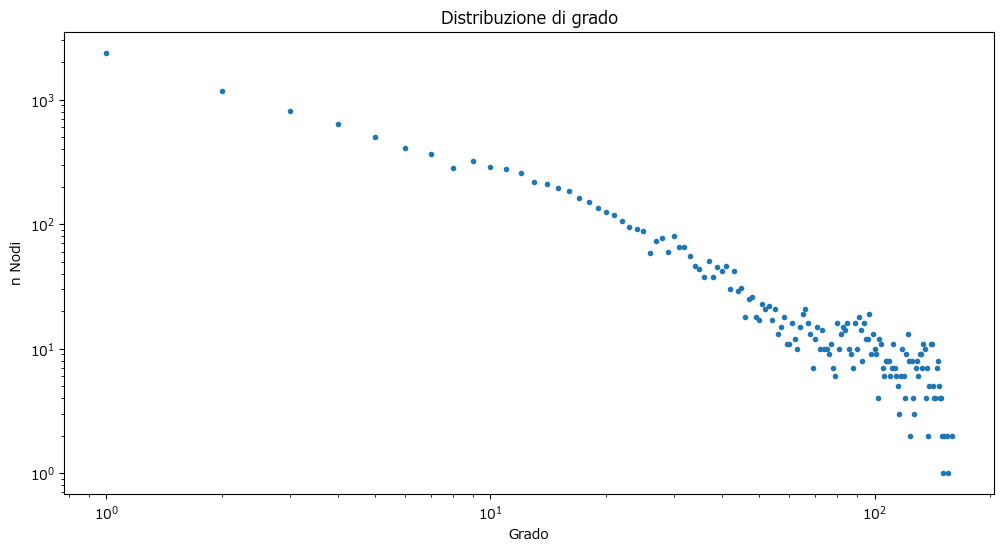
\includegraphics[width=0.45
\textwidth]{../network_analysis/plots/2_2/grDist.png}
\caption{Distribuzione del grado degli artisti}
\label{fig:plotDist}
\end{figure}

Questa asimmetria dei gradi del grafo si mostra maggiormente dalle distribuzioni CDF e CCDF: la probabilità di trovare un artista con grado elevato decresce.

\begin{figure}[H]
\centering
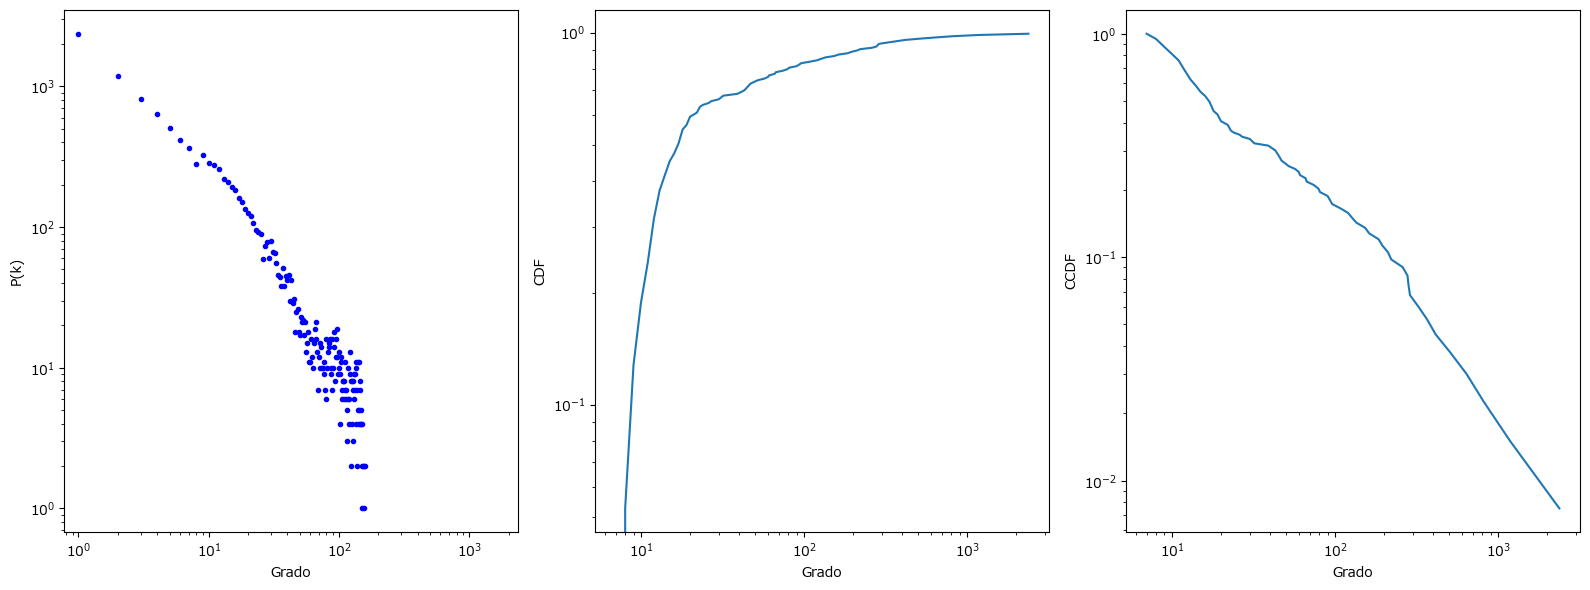
\includegraphics[width=0.45
\textwidth]{../network_analysis/plots/2_2/plotDist.png}
\caption{Distribuzione del grado degli artisti - CDF e CCDF}
\label{fig:plotDist}
\end{figure}

Dato che si tratta di un grafo pesato su due livelli, è interessante mostrare come si comportano i rispettivi pesi con i medesimi grafici. Per cui si illustrano i medesimi grafici ma pesati: qui è evidente come lo Jaccard Ratio risulta più traslato indietro rispetto al Sample corrispondente:

\begin{figure}[H]
\centering
\includegraphics[width=0.45
\textwidth]{../network_analysis/plots/2_2/wGhGrDist.png}
\caption{Distribuzione del grado pesato degli artisti}
\label{fig:plotDist}
\end{figure}

\begin{figure}[H]
\centering
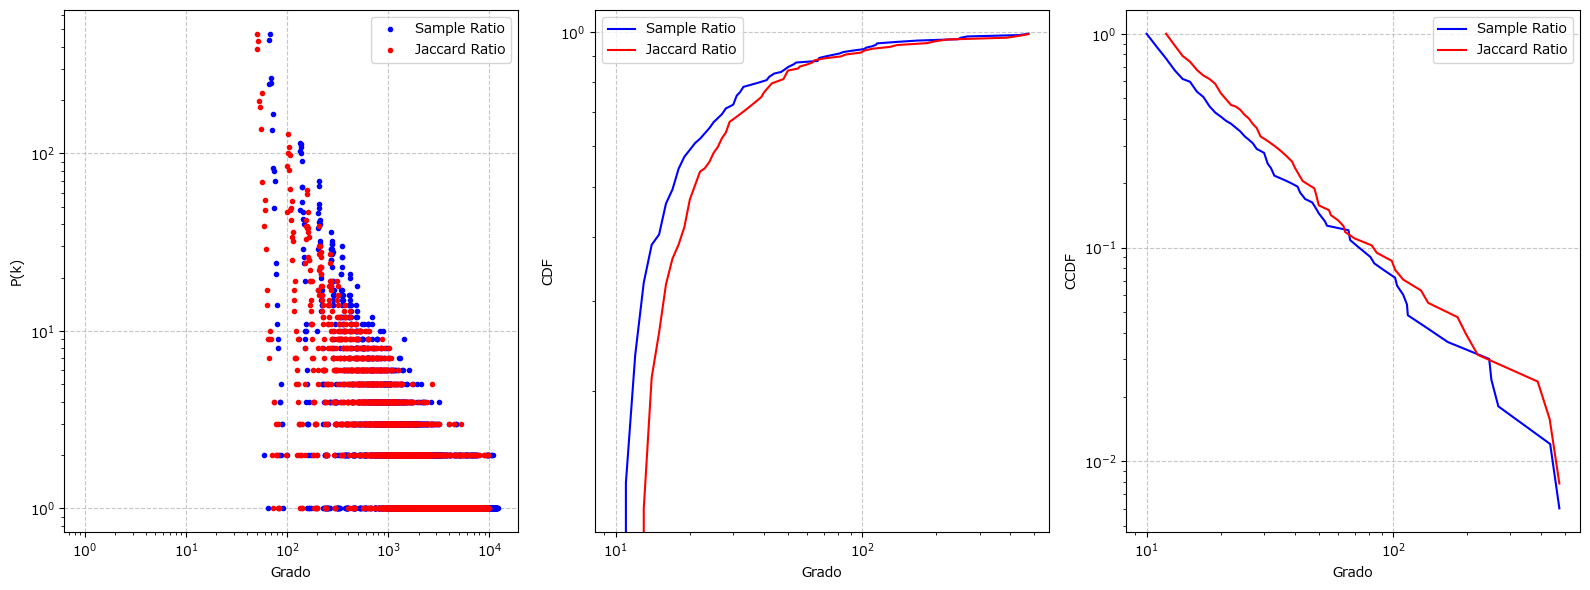
\includegraphics[width=0.45
\textwidth]{../network_analysis/plots/2_2/wPlotDist.png}
\caption{Distribuzione del grado pesato degli artisti - CDF e CCDF}
\label{fig:plotDist}
\end{figure}

\subsection{Comparision with ER}

Lorem ipsum dolor sit amet, consectetur adipiscing elit, sed do eiusmod tempor incididunt ut labore et dolore magna aliqua. Ut enim ad minim veniam, quis nostrud exercitation ullamco laboris nisi ut aliquip ex ea commodo consequat. Duis aute irure dolor in reprehenderit in voluptate velit esse cillum dolore eu fugiat nulla pariatur. Excepteur sint occaecat cupidatat non proident, sunt in culpa qui officia deserunt mollit anim id est laborum.

\subsection{Comparision with BA}

Lorem ipsum dolor sit amet, consectetur adipiscing elit, sed do eiusmod tempor incididunt ut labore et dolore magna aliqua. Ut enim ad minim veniam, quis nostrud exercitation ullamco laboris nisi ut aliquip ex ea commodo consequat. Duis aute irure dolor in reprehenderit in voluptate velit esse cillum dolore eu fugiat nulla pariatur. Excepteur sint occaecat cupidatat non proident, sunt in culpa qui officia deserunt mollit anim id est laborum.

\begin{equation}
  \lim_{n\rightarrow \infty}x= \sum_{i\in B]}\frac{1}{2}
\end{equation}


\section{Task: Open Question}

Lorem ipsum dolor sit amet, consectetur adipiscing elit, sed do eiusmod tempor incididunt ut labore et dolore magna aliqua. Ut enim ad minim veniam, quis nostrud exercitation ullamco laboris nisi ut aliquip ex ea commodo consequat. Duis aute irure dolor in reprehenderit in voluptate velit esse cillum dolore eu fugiat nulla pariatur. Excepteur sint occaecat cupidatat non proident, sunt in culpa qui officia deserunt mollit anim id est laborum.

\section{Discussion}

Lorem ipsum dolor sit amet, consectetur adipiscing elit, sed do eiusmod tempor incididunt ut labore et dolore magna aliqua. Ut enim ad minim veniam, quis nostrud exercitation ullamco laboris nisi ut aliquip ex ea commodo consequat. Duis aute irure dolor in reprehenderit in voluptate velit esse cillum dolore eu fugiat nulla pariatur. Excepteur sint occaecat cupidatat non proident, sunt in culpa qui officia deserunt mollit anim id est laborum.

% The next two lines define the bibliography style to be used, and the bibliography file.
\bibliographystyle{ACM-Reference-Format}
\bibliography{biblio}

\end{document}

